% This file was created with tikzplotlib v0.10.1.
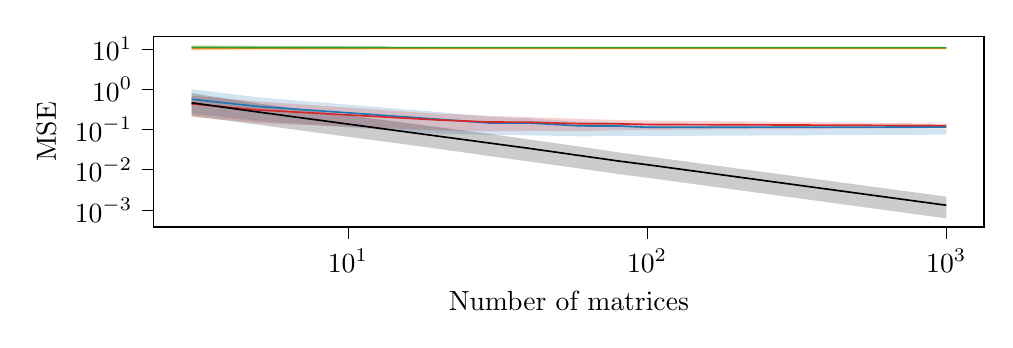
\begin{tikzpicture}

\definecolor{crimson2143940}{RGB}{214,39,40}
\definecolor{darkgray176}{RGB}{176,176,176}
\definecolor{darkorange25512714}{RGB}{255,127,14}
\definecolor{forestgreen4416044}{RGB}{44,160,44}
\definecolor{lightgray204}{RGB}{204,204,204}
\definecolor{steelblue31119180}{RGB}{31,119,180}

\begin{axis}[
width=\columnwidth,
height=4cm,
legend cell align={left},
legend style={
  fill opacity=0.8,
  draw opacity=1,
  text opacity=1,
  at={(0.03,0.03)},
  anchor=south west,
  draw=lightgray204
},
log basis x={10},
log basis y={10},
tick align=outside,
tick pos=left,
x grid style={darkgray176},
xlabel={Number of matrices},
xmin=2.2437647322819, xmax=1337.03857487278,
xmode=log,
xtick style={color=black},
xtick={0.1,1,10,100,1000,10000,100000},
xticklabels={
  \(\displaystyle {10^{-1}}\),
  \(\displaystyle {10^{0}}\),
  \(\displaystyle {10^{1}}\),
  \(\displaystyle {10^{2}}\),
  \(\displaystyle {10^{3}}\),
  \(\displaystyle {10^{4}}\),
  \(\displaystyle {10^{5}}\)
},
y grid style={darkgray176},
ylabel={MSE},
ymin=0.000379717971279199, ymax=20.1375303129162,
ymode=log,
ytick style={color=black},
ytick={1e-05,0.0001,0.001,0.01,0.1,1,10,100,1000},
yticklabels={
  \(\displaystyle {10^{-5}}\),
  \(\displaystyle {10^{-4}}\),
  \(\displaystyle {10^{-3}}\),
  \(\displaystyle {10^{-2}}\),
  \(\displaystyle {10^{-1}}\),
  \(\displaystyle {10^{0}}\),
  \(\displaystyle {10^{1}}\),
  \(\displaystyle {10^{2}}\),
  \(\displaystyle {10^{3}}\)
}
]
\path [fill=steelblue31119180, fill opacity=0.2]
(axis cs:3,1.00111691885235)
--(axis cs:3,0.242662351506986)
--(axis cs:5,0.163221302129445)
--(axis cs:20,0.0780933248622451)
--(axis cs:30,0.073562719369156)
--(axis cs:40,0.0715116867740018)
--(axis cs:60,0.0675163750600415)
--(axis cs:80,0.0688651332729055)
--(axis cs:100,0.0689308857032579)
--(axis cs:1000,0.0743048560270507)
--(axis cs:1000,0.105052514567065)
--(axis cs:1000,0.105052514567065)
--(axis cs:100,0.136630628469856)
--(axis cs:80,0.151747410388139)
--(axis cs:60,0.157045002201535)
--(axis cs:40,0.189221097709762)
--(axis cs:30,0.205596166051169)
--(axis cs:20,0.271233850899762)
--(axis cs:5,0.628482264113363)
--(axis cs:3,1.00111691885235)
--cycle;

\path [fill=darkorange25512714, fill opacity=0.2]
(axis cs:3,12.13555385122)
--(axis cs:3,8.93652083178367)
--(axis cs:5,9.25126149157753)
--(axis cs:20,9.66889083367207)
--(axis cs:30,9.79754417185975)
--(axis cs:40,9.85450545926054)
--(axis cs:60,9.92433898298992)
--(axis cs:80,9.94940436153678)
--(axis cs:100,10.0086614354127)
--(axis cs:1000,10.1934231185474)
--(axis cs:1000,10.3745241955988)
--(axis cs:1000,10.3745241955988)
--(axis cs:100,10.5648394017509)
--(axis cs:80,10.5941642503707)
--(axis cs:60,10.6392962811557)
--(axis cs:40,10.7218086423827)
--(axis cs:30,10.8092916653157)
--(axis cs:20,10.9533699187732)
--(axis cs:5,11.6028123200417)
--(axis cs:3,12.13555385122)
--cycle;

\path [fill=forestgreen4416044, fill opacity=0.2]
(axis cs:3,12.2815776729252)
--(axis cs:3,9.44328359347)
--(axis cs:5,9.79054769703643)
--(axis cs:20,10.1812987877089)
--(axis cs:30,10.2635015903304)
--(axis cs:40,10.3269740172121)
--(axis cs:60,10.3975711261742)
--(axis cs:80,10.43312797331)
--(axis cs:100,10.4650638577213)
--(axis cs:1000,10.6198964124901)
--(axis cs:1000,10.7807681514766)
--(axis cs:1000,10.7807681514766)
--(axis cs:100,10.9531337372961)
--(axis cs:80,10.9732930511024)
--(axis cs:60,11.0264844260148)
--(axis cs:40,11.1207262559774)
--(axis cs:30,11.1683909575603)
--(axis cs:20,11.2761192082818)
--(axis cs:5,11.9139859240684)
--(axis cs:3,12.2815776729252)
--cycle;

\path [fill=crimson2143940, fill opacity=0.2]
(axis cs:3,0.690931467599105)
--(axis cs:3,0.206219207260978)
--(axis cs:5,0.14510210542033)
--(axis cs:20,0.0948519988141808)
--(axis cs:30,0.089681912341369)
--(axis cs:40,0.0918892596422362)
--(axis cs:60,0.092118389580167)
--(axis cs:80,0.0952253421601221)
--(axis cs:100,0.097604956828388)
--(axis cs:1000,0.108470580186441)
--(axis cs:1000,0.139813549239583)
--(axis cs:1000,0.139813549239583)
--(axis cs:100,0.167369321658288)
--(axis cs:80,0.172111214225925)
--(axis cs:60,0.183501078893765)
--(axis cs:40,0.202017108103555)
--(axis cs:30,0.218945976003984)
--(axis cs:20,0.245585349092971)
--(axis cs:5,0.495715555534937)
--(axis cs:3,0.690931467599105)
--cycle;

\path [fill=black, fill opacity=0.2]
(axis cs:3,0.794318934700682)
--(axis cs:3,0.21637240879828)
--(axis cs:5,0.131316283900395)
--(axis cs:20,0.0331722272946312)
--(axis cs:30,0.021649675024175)
--(axis cs:40,0.0162019228464954)
--(axis cs:60,0.0106635138506762)
--(axis cs:80,0.0078405015134601)
--(axis cs:100,0.0063496262976184)
--(axis cs:1000,0.0006226058541201)
--(axis cs:1000,0.0021538830893464)
--(axis cs:1000,0.0021538830893464)
--(axis cs:100,0.0216262414400377)
--(axis cs:80,0.0270677899044086)
--(axis cs:60,0.0373148080352239)
--(axis cs:40,0.0568307965558478)
--(axis cs:30,0.0771502807932365)
--(axis cs:20,0.114242923177177)
--(axis cs:5,0.443383024766154)
--(axis cs:3,0.794318934700682)
--cycle;

\addplot [semithick, steelblue31119180]
table {%
3 0.561803044679663
5 0.372785036853189
20 0.179474625108256
30 0.143976940239739
40 0.144965931008824
60 0.122471664251872
80 0.122251731403312
100 0.113571055810565
1000 0.114853176532061
};
\addlegendentry{SCM}
\addplot [semithick, darkorange25512714]
table {%
3 10.4952751372028
5 10.4100832183256
20 10.3128793582248
30 10.3008149630267
40 10.288634572172
60 10.2887083705405
80 10.2747889284676
100 10.2835187064137
1000 10.281949648189
};
\addlegendentry{LW linear}
\addplot [semithick, forestgreen4416044]
table {%
3 10.89702763455
5 10.8308375664196
20 10.7225329134666
30 10.7137319401956
40 10.7104421615176
60 10.7113947362119
80 10.7038714258237
100 10.7050678575276
1000 10.6998167554028
};
\addlegendentry{OAS}
\addplot [semithick, crimson2143940]
table {%
3 0.431596273303805
5 0.305730000712655
20 0.172086794045216
30 0.152926116067352
40 0.151737695108779
60 0.138622803351817
80 0.137723753115095
100 0.133427856149854
1000 0.124500946921857
};
\addlegendentry{LW nonlinear}
\addplot [semithick, black]
table {%
3 0.460079303501696
5 0.271485128543989
20 0.0682589839891463
30 0.0455971037537456
40 0.0342338614296108
60 0.0223472202386557
80 0.016535800668534
100 0.0133605802455973
1000 0.0013178391989009
};
\addlegendentry{RMT}

\legend{};
\end{axis}

\end{tikzpicture}
